\documentclass[runningheads]{llncs}
\usepackage[T1]{fontenc}
\usepackage{lmodern}
\usepackage[utf8]{inputenc}
\usepackage[spanish,es-noshorthands,es-tabla]{babel}
\usepackage{graphicx}
\usepackage{booktabs}
\usepackage{placeins}
\usepackage{amsmath}
\usepackage{siunitx}
\sisetup{output-decimal-marker={,}, group-separator={.}, detect-all}
\usepackage{tikz}
\usetikzlibrary{arrows.meta,positioning,calc}
\usepackage[hidelinks]{hyperref}
\usepackage{xcolor}
\definecolor{ida}{HTML}{2A78D6}
\definecolor{vuelta}{HTML}{EB6834}
\definecolor{tinta}{HTML}{52514E}

\begin{document}
\renewcommand{\keywordname}{{\bfseries Palabras clave:}}
\renewcommand{\andname}{y}\renewcommand{\lastandname}{\unskip{} y}

\title{Simulación de eventos discretos de la ruta de buses entre el Parque de los Estudiantes y el campus Barcelona de la Universidad de los Llanos}
\titlerunning{Simulación de la ruta Parque-Campus Barcelona}

\author{Johan Sebastián Forero Agudelo \and Santiago Barrera Meza \and Juan Diego Vélez González}
\authorrunning{J. S. Forero Agudelo et al.}

\institute{Ingeniería de Sistemas, Universidad de los Llanos, Villavicencio, Colombia\\
Simulación Computacional, Prof. Angel Alfonso Cruz Roa\\
\email{\{jsforero.agudelo, sbarrera.meza, jdvelez\}@unillanos.edu.co}}

\maketitle

\begin{abstract}
La ruta institucional que une el Parque de los Estudiantes, en el centro de Villavicencio, con el campus Barcelona de la Universidad de los Llanos opera con horario fijo sobre un corredor sujeto al tráfico urbano y a una demanda concentrada en las horas pico académicas. Se presenta un modelo de simulación de eventos discretos en AnyLogic que representa la operación en ambos sentidos: salidas cada 20 minutos de 5:20 a 22:00, nueve paraderos de ida y ocho de vuelta, cinco buses de 41 puestos sentados (51 con pasajeros de pie), tiempos de abordaje y descenso, y tiempos de recorrido por tramo y franja. Estos tiempos se obtuvieron de Google Maps durante una semana hábil y se modelaron con distribuciones triangulares. La demanda se generó con procesos de Poisson por franja. Una salida sin bus disponible sale tarde y no se cancela. El modelo reproduce los tiempos de entrada con un error de a lo sumo 2,2\,\%. Con 30 réplicas se compararon la operación actual y un inicio de semestre con 40\,\% más de demanda, dos buses en mantenimiento y 35\,\% más de tiempo en la vía al campus. En la operación actual la espera media en parada es de 11,5 minutos y el viaje puerta a puerta dura 35,8 minutos. En el inicio de semestre suben a 58,7 y 87,6 minutos, y las salidas acumulan un retraso medio de 3,2 horas. Con cinco buses la ruta cumple su horario, pero con tres no lo cumple.
\keywords{Simulación de eventos discretos \and Transporte universitario \and AnyLogic \and Distribución triangular \and Análisis de escenarios.}
\end{abstract}

\section{Introducción}

\textbf{Motivación.} La Universidad de los Llanos ofrece rutas institucionales de bus entre distintos barrios de Villavicencio y su sede principal, el campus Barcelona, ubicado a unos 12\,km del centro sobre la vía a Puerto López. La ruta Parque recorre el corredor de la carrera 33 y la vía nacional hasta la entrada del campus. Para quienes la usan, la espera en el paradero y la duración del viaje inciden en la puntualidad a clases y en la hora de regreso al centro.

\textbf{Problema.} La ruta tiene un horario fijo, cada 20 minutos en ambos sentidos de 5:20 a 22:00, pero la demanda no es uniforme: se concentra antes de las clases de la mañana, al mediodía y al final de la tarde. Además, el tráfico urbano hace variar los tiempos de recorrido según la hora. No se sabe cuánto esperan los pasajeros, cuánto dura el viaje completo ni qué tan llenos van los buses en cada tramo. Tampoco se sabe cómo cambian estos indicadores en las primeras semanas de semestre, cuando la demanda crece y coincide con buses en mantenimiento.

\textbf{Justificación.} Experimentar sobre el sistema real (retirar buses o cambiar horarios) es costoso y afecta a los usuarios. Un modelo de simulación permite evaluar esas decisiones sin intervenir la operación y cuantificar con intervalos de confianza su efecto sobre el servicio~\cite{law2015,banks2010}. La simulación se ha usado para estudiar la operación de buses, la regularidad de los intervalos y la carga por tramo~\cite{cats2010,ceder2016}. Se eligió la simulación de eventos discretos porque el estado del sistema solo cambia en instantes puntuales, como la llegada de un pasajero, la salida de un bus o su arribo a un paradero.

\textbf{Objetivos.} El objetivo general es evaluar con simulación de eventos discretos el desempeño de la ruta en dos escenarios de operación. Para ello se construye en AnyLogic un modelo de la ruta en ambos sentidos, se modelan los tiempos de recorrido por tramo y franja con distribuciones estimadas a partir de datos, se estiman el tiempo de espera en parada, el tiempo puerta a puerta y el factor de ocupación por tramo, y se compara la operación actual con un escenario de inicio de semestre.

\section{Metodología}

Se siguieron las etapas de un estudio de simulación~\cite{law2015,banks2010}: formulación del problema, recolección y análisis de datos de entrada, modelo conceptual, implementación, verificación y validación, diseño experimental y análisis de resultados. La implementación se hizo en AnyLogic~8.9 PLE~\cite{borshchev2013}, combinando la biblioteca de modelado de procesos (fuentes y bloques de espera para los pasajeros) con diagramas de estados para los buses.

\textbf{Esquema del sistema.} La Fig.~\ref{fig:esquema} resume el modelo. Los pasajeros de ida llegan a ocho paraderos (del Parque a la EDS Primax Ocoa) y todos descienden en Barcelona. Los de vuelta llegan solo a Barcelona y descienden en los siete paraderos de regreso, que no incluyen la EDS. Cada bus pasa por cuatro estados: \emph{Libre} en un extremo, \emph{EnParada}, \emph{EnTramo} y \emph{Alistando} (5\,min en cada extremo). Al terminar un viaje queda libre en el extremo al que llegó, así que alterna ida y vuelta sin viajes vacíos.

\begin{figure}[t]
\centering
\resizebox{\linewidth}{!}{%
\begin{tikzpicture}[x=1cm,y=1cm,font=\scriptsize,
  par/.style={circle,draw=#1,fill=white,line width=.8pt,inner sep=1.6pt},
  caja/.style={draw=tinta,rounded corners=2pt,align=center,inner sep=3pt,font=\scriptsize}]
  \def\xs{0,0.53,1.15,1.64,2.6,3.08,4.43,5.39,11.0}
  \foreach \x [count=\i] in \xs { \coordinate (I\i) at (\x,0); }
  \draw[ida,line width=1.4pt,-{Latex[length=2mm]}] (0,0) -- (11,0);
  \draw[vuelta,line width=1.4pt,-{Latex[length=2mm]}] (11,-.9) -- (0,-.9);
  \foreach \x [count=\i] in \xs { \node[par=ida] at (\x,0) {}; }
  \foreach \x in {11,4.43,3.08,2.6,1.64,1.15,0.53,0} { \node[par=vuelta] at (\x,-.9) {}; }
  \node[above=2pt,anchor=south west,rotate=35] at (0,0.05) {Parque};
  \node[above=2pt,anchor=south west,rotate=35] at (0.53,0.05) {Unicentro};
  \node[above=2pt,anchor=south west,rotate=35] at (1.15,0.05) {Tecniguayas};
  \node[above=2pt,anchor=south west,rotate=35] at (1.64,0.05) {C. Industrial};
  \node[above=2pt,anchor=south west,rotate=35] at (2.6,0.05) {Makro};
  \node[above=2pt,anchor=south west,rotate=35] at (3.08,0.05) {La Alborada};
  \node[above=2pt,anchor=south west,rotate=35] at (4.43,0.05) {U. Cooperativa};
  \node[above=2pt,anchor=south west,rotate=35] at (5.39,0.05) {EDS Ocoa};
  \node[above=2pt,anchor=south west,rotate=35] at (11,0.05) {Barcelona};
  \node[ida,anchor=west] at (6.2,.25) {Ida: suben en 8 paraderos, bajan todos en Barcelona};
  \node[vuelta,anchor=west] at (5.3,-1.15) {Vuelta: suben en Barcelona, bajan en 7 paraderos};
  \draw[tinta,dashed] (8.2,-.15) -- (8.2,-.75) node[midway,right,tinta] {vía al campus};
  \node[caja] (src) at (0.9,-2.35) {Fuentes Poisson\\por franja};
  \node[caja] (wait) at (3.4,-2.35) {Espera en\\paradero (FIFO)};
  \node[caja] (bus) at (6.25,-2.35) {Bus: abordaje 3\,s/pax,\\descenso 2\,s/pax, 10\,s fijos};
  \node[caja] (tramo) at (9.6,-2.35) {Tramo: triangular\\$\times 1{,}1$ por franja};
  \draw[-{Latex[length=1.6mm]},tinta] (src) -- (wait);
  \draw[-{Latex[length=1.6mm]},tinta] (wait) -- (bus);
  \draw[-{Latex[length=1.6mm]},tinta] (bus) -- (tramo);
  \draw[-{Latex[length=1.6mm]},tinta] (tramo.south) -- ++(0,-.3) -| (bus.south) node[pos=.25,below] {siguiente paradero};
\end{tikzpicture}}
\caption{Esquema del sistema simulado. Arriba, la ruta con distancias a escala. Abajo, el flujo de entidades del modelo de eventos discretos.}
\label{fig:esquema}
\end{figure}

\textbf{Reglas de operación.} Las salidas se programan cada 20\,min de 5:20 a 22:00 en ambos sentidos, 51 por sentido. Al iniciar el día, la mitad de la flota (redondeada hacia arriba) está en el Parque y el resto en Barcelona. A la hora programada, la salida toma el primer bus libre del extremo correspondiente. Si no hay bus, sale tarde en cuanto llega uno y recoge a quienes estén esperando. Ninguna salida se cancela ni se une a la siguiente. En la vuelta el bus aborda a todos los que esperan hasta completar 51 pasajeros.

\textbf{Tiempos de servicio.} La detención en un paradero es de 10\,s fijos más 3\,s por pasajero que aborda y 2\,s por pasajero que desciende, valores dentro de los rangos que reporta el manual de capacidad del transporte público~\cite{tcqsm2013}. En movimiento, el bus es un 10\,\% más lento que un automóvil. La ruta es casi recta y la mayor diferencia viene de las paradas, que se modelan aparte.

\section{Conjunto de datos}

Se usaron dos fuentes. La primera es el horario y la lista de paraderos publicados por la universidad para la ruta Parque. La segunda son los tiempos habituales de conducción de Google Maps para cada uno de los 15 tramos (8 de ida y 7 de vuelta), consultados con hora de salida a las 5:30 (pico de la mañana), 10:00 (valle) y 17:30 (pico de la tarde) para los cinco días hábiles de una semana. De cada tramo y franja se conservó el tiempo promedio de la semana y los valores mínimo y máximo observados. La Tabla~\ref{tab:datos} muestra ejemplos, incluidos los dos tramos de la vía al campus, que concentran la mayor parte del tiempo y de la variabilidad.

\begin{table}[t]
\centering
\caption{Ejemplos del conjunto de datos de tiempos por tramo (minutos en automóvil).}
\label{tab:datos}
\setlength{\tabcolsep}{4pt}
\begin{tabular}{llrlrrr}
\toprule
Sentido & Tramo & km & Franja & Prom. & Mín. & Máx.\\
\midrule
Ida & 1: Parque $\to$ Unicentro & 0,55 & Pico 17:30 & 4,00 & 2 & 6\\
Ida & 8: EDS Ocoa $\to$ Barcelona & 5,90 & Pico 5:30 & 8,92 & 7 & 12\\
Ida & 8: EDS Ocoa $\to$ Barcelona & 5,90 & Pico 17:30 & 10,00 & 8 & 12\\
Vuelta & 1: Barcelona $\to$ U. Coop. & 6,90 & Valle 10:00 & 12,25 & 9 & 16\\
Vuelta & 7: Unicentro $\to$ Parque & 0,80 & Valle 10:00 & 4,92 & 3 & 7\\
\bottomrule
\end{tabular}
\end{table}

\textbf{Análisis de entrada.} Para cada tramo y franja se tiene un mínimo, un máximo y un promedio, así que se eligió la distribución triangular, que es la recomendada cuando los datos son escasos y se conocen esos tres valores~\cite{law2015}. La moda se fijó como $c = 3\bar{x} - a - b$ (recortada a $[a,b]$), de modo que la media teórica $(a+b+c)/3$ coincide con el promedio medido. Cuando el mínimo y el máximo coincidían, se abrió el intervalo $\pm 0{,}5$\,min para conservar algo de variabilidad. Los datos son resúmenes semanales y no observaciones individuales. Por eso no fue posible ajustar ni contrastar distribuciones Normal o Lognormal, ni aplicar pruebas formales de independencia, y esta es la principal limitación del estudio.

La estabilidad se analizó comparando franjas (Fig.~\ref{fig:entrada}). En la ida, el recorrido completo pasa de 21,1\,min en el pico de la mañana a 28,5\,min en el de la tarde (+35\,\%). En la vuelta, el valle y la tarde son casi iguales. Por esta diferencia, las horas pico y valle se modelan por separado. Los tramos urbanos varían poco en valor absoluto, mientras que los de la vía al campus tienen rangos de 4 a 7\,min.

\begin{figure}[t]
\centering
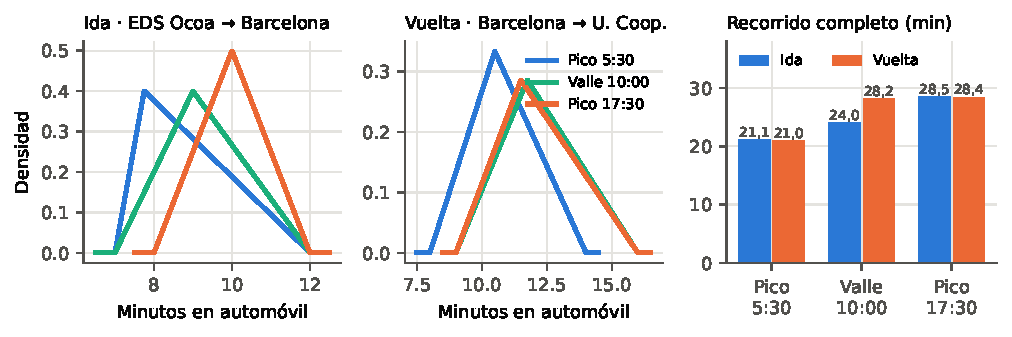
\includegraphics[width=\linewidth]{figuras/entrada.pdf}
\caption{Izquierda y centro: distribuciones triangulares ajustadas para los tramos de la vía al campus. Derecha: tiempo total del recorrido por franja, que muestra la diferencia entre horas pico y valle.}
\label{fig:entrada}
\end{figure}

\textbf{Demanda.} No se contó con conteos de pasajeros, por lo que la demanda se generó de forma sintética con procesos de Poisson de tasa constante por franja. Las horas pico son de 5:30 a 7:00, de 11:00 a 14:00 y de 17:30 a 19:00. En la ida se usaron 140, 90 y 45 pasajeros/h en el pico de la mañana, el del mediodía y el valle, y 30 en la tarde y la noche, repartidos entre paraderos con pesos de 0,30 para el Parque, 0,15 para Unicentro y 0,05 a 0,10 para los demás. En la vuelta se usaron 130 y 150 pasajeros/h en Barcelona al mediodía y en la tarde, 45 en el valle y 30 en la noche, a partir de las 7:40. Las llegadas terminan a las 21:55, antes de la última salida. Los destinos de la vuelta siguen probabilidades fijas, con un 35\,\% hasta el Parque.

\section{Diseño experimental}

\textbf{Escenarios.} El escenario E1 es la operación actual, con cinco buses, la demanda base y los tiempos medidos. El escenario E2 es el inicio de semestre, con la demanda multiplicada por 1,4, dos buses en mantenimiento (tres en servicio) y los tramos de la vía al campus (ida 8 y vuelta 1) un 35\,\% más lentos por congestión. Cada réplica simula un día de servicio y se prolonga hasta completar 48\,h, para que terminen los viajes atrasados. Al final el sistema se vacía, así que las réplicas son independientes y no se requiere periodo de calentamiento.

\textbf{Partición de los datos de simulación.} Las corridas se dividieron en tres grupos con semillas disjuntas. \emph{Entrenamiento}: 10 réplicas piloto por escenario para estimar la varianza de la espera media y calcular el número de réplicas necesario para un error relativo del 5\,\% con 95\,\% de confianza, $n = \lceil n_0 (h/(\gamma\bar{x}))^2\rceil$~\cite{law2015}. Resultó $n=10$ para E1 y $n=18$ para E2, y se adoptó $n=30$ para ambos. \emph{Validación}: 30 réplicas de E1 en la implementación en Python para contrastar el tiempo en movimiento simulado con los tiempos de Google Maps (Tabla~\ref{tab:validacion}). \emph{Prueba}: 30 réplicas por escenario con números aleatorios comunes en la implementación en Python, que sigue las mismas reglas del modelo de AnyLogic. Los escenarios se comparan con la prueba $t$ pareada.

\begin{table}[t]
\centering
\caption{Validación: tiempo de recorrido en movimiento simulado (dividido entre 1,1) frente a la suma de los promedios de Google Maps, en minutos.}
\label{tab:validacion}
\setlength{\tabcolsep}{5pt}
\begin{tabular}{llrrrr}
\toprule
Sentido & Franja & Google Maps & Simulado & Dif. & Detenido en paradas\\
\midrule
Ida & Pico mañana & 21,08 & 21,35 & +1,3\,\% & 5,10\\
Ida & Valle & 24,00 & 24,04 & +0,2\,\% & 2,35\\
Ida & Pico tarde & 28,50 & 28,25 & $-$0,9\,\% & 3,23\\
Vuelta & Pico mañana & 21,00 & 21,46 & +2,2\,\% & 0,00\\
Vuelta & Valle & 28,17 & 28,06 & $-$0,4\,\% & 2,12\\
Vuelta & Pico tarde & 28,42 & 28,51 & +0,3\,\% & 4,78\\
\bottomrule
\end{tabular}
\end{table}

\textbf{Medidas de desempeño.} En cada réplica se registra el tiempo medio de espera en parada, que va desde la llegada del pasajero hasta su abordaje, y el tiempo medio puerta a puerta, que va desde la llegada al paradero hasta el descenso. También se registra el factor de ocupación por tramo, calculado como pasajeros a bordo sobre los 41 puestos sentados, de modo que un valor mayor que 1 indica pasajeros de pie. Como medidas secundarias se registran el retraso medio y el retraso máximo de salida y los pasajeros sin servicio al cierre.

\textbf{Verificación.} La lógica se verificó trazando las salidas de un día y comprobando que ningún bus supera los 51 pasajeros, que con demanda nula no hay esperas y que se realizan las 102 salidas del día, aunque alguna salga tarde. El modelo también se implementó en Python con la biblioteca SimPy, con la misma lógica de operación. En una versión anterior de las reglas, las dos implementaciones difirieron en cerca del 4\,\% en espera, tiempo puerta a puerta y ocupación.

\section{Resultados}

La Tabla~\ref{tab:resultados} resume las 30 réplicas de prueba por escenario. Todas las diferencias entre escenarios son significativas ($p<10^{-23}$, prueba $t$ pareada). En ningún escenario quedan pasajeros sin servicio, porque todas las salidas se realizan, aunque sea tarde.

\begin{table}[t]
\centering
\caption{Medidas de desempeño: media e intervalo de confianza del 95\,\% (30 réplicas por escenario).}
\label{tab:resultados}
\setlength{\tabcolsep}{6pt}
\begin{tabular}{lrr}
\toprule
Medida & E1: Actual & E2: Inicio de semestre\\
\midrule
Espera en parada, total (min) & 11,49 $\pm$ 0,13 & 58,69 $\pm$ 2,08\\
\quad ida (min) & 10,70 $\pm$ 0,12 & 31,55 $\pm$ 1,36\\
\quad vuelta (min) & 12,26 $\pm$ 0,18 & 84,86 $\pm$ 3,65\\
Puerta a puerta, total (min) & 35,84 $\pm$ 0,15 & 87,63 $\pm$ 2,12\\
\quad ida (min) & 33,62 $\pm$ 0,19 & 58,78 $\pm$ 1,37\\
\quad vuelta (min) & 37,97 $\pm$ 0,26 & 115,46 $\pm$ 3,67\\
Factor de ocupación medio & 0,325 $\pm$ 0,003 & 0,456 $\pm$ 0,004\\
Tramos con pasajeros de pie (\%) & 3,4 $\pm$ 0,3 & 17,2 $\pm$ 0,5\\
Retraso medio de salida (min) & 0,05 $\pm$ 0,01 & 190,4 $\pm$ 1,7\\
Retraso máximo de salida (min) & 2,2 $\pm$ 0,3 & 382,3 $\pm$ 3,4\\
\bottomrule
\end{tabular}
\end{table}

\textbf{Operación actual.} La espera media de 11,5\,min es algo mayor que la mitad del intervalo entre salidas (10\,min), así que en la mayoría de las salidas suben todos los que esperan. Las salidas son prácticamente puntuales (retraso medio de 0,05\,min). El viaje puerta a puerta es de 36\,min, de los cuales unos 24 corresponden al recorrido. La ocupación media es del 32\,\% y solo el 3\,\% de los tramos lleva pasajeros de pie, concentrados en la salida de Barcelona en las horas pico de la vuelta (Fig.~\ref{fig:ocupacion}).

\textbf{Inicio de semestre.} El ciclo completo de un bus (ida, vuelta y alistamientos) dura unos 70\,min, así que tres buses solo alcanzan a ofrecer una salida en cada sentido cada 23\,min, y el horario pide una cada 20\,min. Como ninguna salida se cancela, cada una espera a que llegue un bus y el retraso se acumula durante el día: en promedio 3,2\,h, y la salida programada a las 22:00 parte hacia las 4:20 de la madrugada. La cola en Barcelona crece al mediodía y en la tarde (Fig.~\ref{fig:espera}). La espera media se multiplica por 5,1 en total y por 6,9 en la vuelta, y el 17\,\% de los tramos lleva pasajeros de pie.

\begin{figure}[t]
\centering
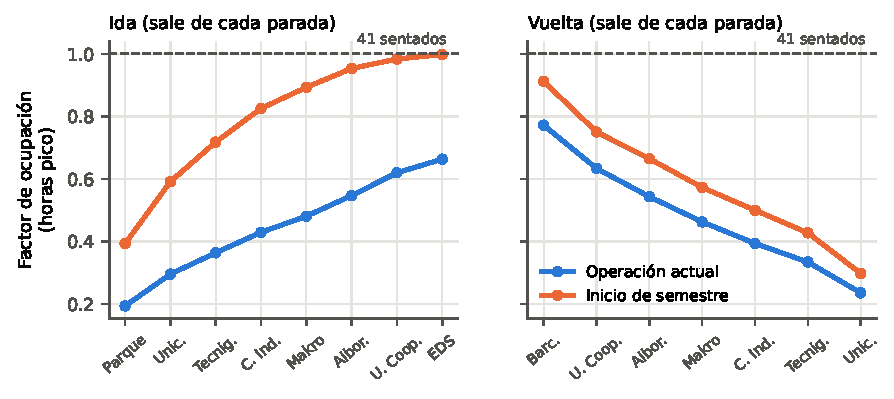
\includegraphics[width=\linewidth]{figuras/ocupacion_tramo.pdf}
\caption{Factor de ocupación medio en horas pico al salir de cada paradero (implementación en Python). La línea discontinua marca los 41 puestos sentados.}
\label{fig:ocupacion}
\end{figure}

\begin{figure}[t]
\centering
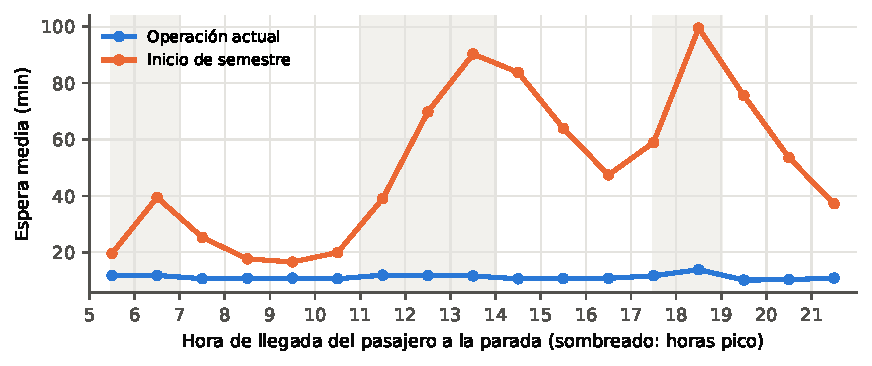
\includegraphics[width=\linewidth]{figuras/espera_por_hora.pdf}
\caption{Espera media según la hora de llegada al paradero (implementación en Python, 10 réplicas por escenario). Las bandas sombreadas son las horas pico.}
\label{fig:espera}
\end{figure}

\FloatBarrier
\section{Conclusiones}

El modelo reproduce los tiempos de recorrido de entrada con un error de a lo sumo 2,2\,\% y muestra que, con cinco buses y salidas cada 20\,min de 5:20 a 22:00, la ruta Parque atiende la demanda base con salidas puntuales, esperas cercanas a la mitad del intervalo y ocupación moderada. Con dos buses menos, el ciclo de cada bus supera el intervalo programado. Las salidas acumulan horas de retraso y el servicio se extiende hasta la madrugada en la época de mayor demanda, así que lo que limita la ruta es la cantidad de buses disponibles. Para el inicio de semestre conviene programar el mantenimiento fuera de las primeras semanas o asignar buses de otras rutas en la vuelta del mediodía y de la tarde. Como trabajo futuro se propone reemplazar la demanda sintética por conteos de campo, medir tiempos de recorrido individuales para ajustar y contrastar otras distribuciones, y evaluar el escenario alterno de mayor frecuencia en horas pico.

\begin{thebibliography}{8}

\bibitem{law2015}
Law, A.M.: Simulation Modeling and Analysis. 5th edn. McGraw-Hill, New York (2015)

\bibitem{banks2010}
Banks, J., Carson, J.S., Nelson, B.L., Nicol, D.M.: Discrete-Event System Simulation. 5th edn. Pearson, Upper Saddle River (2010)

\bibitem{borshchev2013}
Borshchev, A.: The Big Book of Simulation Modeling: Multimethod Modeling with AnyLogic 6. AnyLogic North America, Chicago (2013)

\bibitem{tcqsm2013}
Kittelson \& Associates, et al.: Transit Capacity and Quality of Service Manual. 3rd edn. TCRP Report 165. Transportation Research Board, Washington, DC (2013)

\bibitem{cats2010}
Cats, O., Burghout, W., Toledo, T., Koutsopoulos, H.N.: Mesoscopic modeling of bus public transportation. Transportation Research Record \textbf{2188}, 9-18 (2010)

\bibitem{ceder2016}
Ceder, A.: Public Transit Planning and Operation: Modeling, Practice and Behavior. 2nd edn. CRC Press, Boca Raton (2016)

\end{thebibliography}

\end{document}
